\section{Appendix: Convective Suppression due to Rotation and Magnetic Fields}
\label{sec:c5_suppression}

In this appendix, we detail our calculations of rotating and magnetized simmering WDs.  In general, their inclusion greatly complicates the treatment of convection inside a star by introducing non-spherically symmetric alterations to the convective structure, non-ideal magnetohydrodynamic (MHD) effects, and coupling, generally non-local, between the magnetic field, rotation profile and convective structure.  Because the purpose of this work is to provide only rough estimates for the effects of rotation and magnetic fields, a full treatment of these is well beyond its scope.  We instead implement the simple modifications to \deltanab\ and \vconv\ derived by \citeal{stev79}.

\citeal{stev79} linearizes the Boussinesq MHD equations.  By assuming the convection is Rayleigh-B\'{e}nard (planar geometry, with uniform vertical gravitational field and background temperature gradient) and that all perturbations to fluid variables can be written as sums of modes $\propto\exp({\bf k}\cdot{\bf x} + \sigma t)$, he obtains the dispersion relation

\begin{eqnarray}
\sigma^4 + \sigma^2\left(2\frac{({\bf k}\cdot{\bf B})^2}{4\pi\rho} + \frac{(2\boldsymbol{\Omega}\cdot{\bf k})^2}{k^2} + N_*^2\frac{k_\perp^2}{k^2}\right) + \nonumber \\
\left(\frac{({\bf k}\cdot{\bf B})^2}{4\pi\rho}\right)^2 + \left(\frac{({\bf k}\cdot{\bf B})^2}{4\pi\rho}\right)N_*^2\frac{k_\perp^2}{k^2} = 0
\label{eq:c5_stev79dispersion}
\end{eqnarray}

\noindent in the limit of zero magnetic dissipation; $\sigma$ is the temporal growth rate of a given mode and $N_*^2 = -g\delta\Delta/H_P$ is the Brunt-V\"{a}is\"{a}l\"{a} (buoyancy) frequency.  \citeal{stev79} then assumes that, for modes with $\sigma > 0$, the non-linear terms in the Boussinesq equations eventually limit their growth, leading to $\sigma$ equalling the nonlinear cascade rate $\sim kv$ at the convective steady state \citep{barkdl14}.  He also assumes convection at steady state is dominated by the mode that transports the greatest heat flux.  The former assumption leads to a relationship between $\sigma$, the mode velocity $v$ (equivalent to \vconv) and wavevector ${\bf k}$:

\eqbegin
\sigma = v/k.
\label{eq:c5_stev79saturation}
\eqend

\noindent Eqns. \ref{eq:c5_stev79dispersion} and \ref{eq:c5_stev79saturation} can then be combined with the mode heat flux

\eqbegin
F = \frac{\rho c_PT}{g\delta}\frac{\sigma^2}{k^2}\left(\sigma + \frac{1}{\sigma}\frac{({\bf k}\cdot{\bf B})^2}{4\pi\rho}\right)
\label{eq:c5_stev79flux}
\eqend

\noindent to determine the one that dominates thermal transport.

For non-rotating, unmagnetized WDs, this formulation reproduces Eqns. \ref{eq:c5_vconv_mlt} and \ref{eq:c5_superad_dev} from MLT, except with prefactor coefficients:

\eqbegin
\Fconv = \frac{4\pi}{25}\left(\frac{5}{2}\right)^{5/2}\frac{\rho c_PT}{\gacc\delta l_m} \vconv^3,
\label{eq:c5_vconv_stev}
\eqend

\eqbegin
\dnabconv = \frac{25\pi^2}{6}\frac{\vconv^2}{\gacc\delta}\frac{H_P}{l_m^2}.
\label{eq:c5_superad_dev_stev}
\eqend

\noindent \citeal{stev79} point out that, for his formulation to reproduce the current age, luminosity and effective temperature of the Sun within a 1D stellar evolution model, it must be calibrated by using $l_m \approx 3H_P$.  In order to be consistent with our non-rotating and unmagnetized results from before, we shall contine to use Eqns. \ref{eq:c5_vconv_mlt} and \ref{eq:c5_superad_dev} rather than Eqns. \ref{eq:c5_vconv_stev} and \ref{eq:c5_superad_dev_stev} in Sec. \ref{ssec:c5_rotmag}.  We consider the result of using these modified coefficients in Sec. \ref{ssec:c5_sensitive_apdx}.

%leading to Eqns. \ref{eq:vconv_stev_hp} and \ref{eq:superad_dev_stev_hp}

For WDs that are rotating or magnetized, \citeal{stev79} finds that his $\Delta$ and \vconv\ can be written as multiplicative factors of the \dnabconv\ and \vconv\ of Eqns. \ref{eq:c5_vconv_stev} and \ref{eq:c5_superad_dev_stev} (using the same \Fconv).  As such, we define \vconvzero\ and \dnabconvzero\ as the convective velocity and temperature gradient calculated assuming \textit{no} rotation or magnetic field.

To further simplify our estimates, we shall assume that the rotation is solid-body and magnetic fields vary slowly over a scale height, and we will consider rotation separately from magnetic fields.  The former is enforced by our use of \citeal{stev79}'s model, since its Rayleigh-B\'{e}nard setup assumes $\boldsymbol{\Omega}$ and ${\bf B}$ are constant over its vertical lengthscale ($H_P$).  At least for rotation, it is also a plausible representation of merger remnant cores, which tend to eliminates differential rotation during post-merger viscous evolution.  Considering rotation and magnetic fields separately allows us to independently gauge the relative importance of each to the runaway.  \citeal{stev79}'s theory also does not include coupling between rotation, convection and magnetic fields.  This neglects, in particular, magnetic field amplification by convective dynamos, which will be discussed further in Sec. \ref{ssec:c5_runaway_mhd}.

\subsection{Simmering of Rotating White Dwarfs}
\label{ssec:c5_runaway_rot}

The exact solution in the rotating case is given by \citeal{stev79} 

\begin{eqnarray}
\frac{\dnabrot}{\dnabconvzero} + \frac{6}{25\pi^2}\rossby^2 &=& \left(\frac{\dnabrot}{\dnabconvzero}\right)^{5/2} \nonumber \\
\frac{\vconv}{\vconvzero} &=& \left(\frac{\dnabrot}{\dnabconvzero}\right)^{-1/4}
\label{eq:c5_rot_exactsoln}
\end{eqnarray}

\noindent where Rossby number

\eqbegin
\rossby = \frac{\vconvzero}{2\Omega l_m} = \frac{\vconvzero}{2\Omega H_P}
\label{eq:c5_rossbynumber}
\eqend

\noindent is a proxy for the ratio between convective and rotational velocities in the convection zone.\footnote{Like \cite{barkdl14}, we assume ${\bf g}||\boldsymbol{\Omega}$ for our calculations; in the case where the two are misaligned, the convective suppression is reduced by a factor ${\bf g}\cdot \boldsymbol{\Omega}/g\Omega$.}  \citeal{stev79} (their Eqn. 43) provide approximations to Eqn. \ref{eq:c5_rot_exactsoln} in the limits of very large and very small \rossby\ (their Eqns. 42 - 43), and in lieu of solving for $\dnabrot/\dnabconvzero$ during integration, we use the approximation

\eqbegin
\frac{\dnabrot}{\dnabconvzero} \approx \left(1 + \left(0.23\rossby^{-4/5}\right)^2\right)^{1/2},
\label{eq:c5_rot_nabrat_apx}
\eqend

\noindent where

\eqbegin
\frac{\dnabrot}{\dnabconvzero}  \approx 0.23\rossby^{-4/5}
\label{eq:c5_rot_nabrat_apx_low}
\eqend

\noindent is the \citeal{stev79} approximation for $\dnabrot/\dnabconvzero$ for $\rossby \ll 1$.\footnote{Using a quadrature averaging of the \citeal{stev79} $\rossby \ll 1$ and $\rossby \gg 1$ expressions is impossible because they do not cross each other.}   Eqn. \ref{eq:c5_rot_nabrat_apx} is accurate to within 3\% of the exact $\dnabrot/\dnabconvzero$ for all \rossby, and $\vconv/\vconvzero = (\dnabrot/\dnabconvzero)^{-1/4}$ to within 1\%.  Eqn. \ref{eq:c5_rot_nabrat_apx_low} can be approximated by $\dnabrot \sim \delta^{-1}(H_P\Omega/c_s)(\vconv/c_s)$, which can be compared to a na\"{i}ve implementation of the (1D analog of the) Solberg-H{\o}iland stability criterion, $\Delta_\mrm{Solberg} \sim \delta^{-1}(H_P\Omega/c_s)^2$ (eg. \citealt{tass00} Sec. 3.4.2).  The replacement of one $H_P\Omega/c_s$ term with $\vconv/c_s$ accounts for the lack of suppression along the axis of rotation, and the turbulent cascade of polar convection into modes orthogonal to the rotation axis in the nonlinear regime \citep{barkdl14}.

%In the limits of very large and very small \rossby, Eqn. \ref{eq:rot_exactsoln} can be approximated by

%\eqbegin
%\dnabconv =
%    \begin{cases}
%      \dnabconvzero(1 + 1/(62\rossby^2)), & \rossby \gg 1 \\
%      0.23\rossby^{-4/5}\dnabconvzero, & \rossby \ll 1.
%    \end{cases}
%\label{eq:rot_approxsoln_dnab}
%\eqend

%\eqbegin
%\vconv =
%    \begin{cases}
%      \vconvzero(1 - 1/(242\rossby^2), & \rossby \gg 1 \\
%      1.5\rossby^{1/5}\vconvzero, & \rossby \ll 1.
%    \end{cases}
%\label{eq:rot_approxsoln_dnab}
%\eqend

Notably, this formulation has been tested in the $\rossby \ll 1$ limit by \cite{barkdl14}, who show through simulations of rotating Rayleigh-B\'{e}nard convection that $\dnabrot \propto \Omega^{4/5}$ and $\vconv \propto \Omega^{-1/5}$ over $10^{-4} \lesssim \rossby \lesssim 10^{-1}$, consistent with \citeal{stev79}.  While not a simulation of a convecting star, this lends credence to \citeal{stev79}'s assumptions for convective transport and nonlinear mode saturation.

Conservation of angular momentum and solid-body rotation are both assumed for the entirety of the runaway, constraining $\Omega$ such that it only needs to be specified for one model along the simmering track; we choose the one at the start of simmering.  This is done by specifying the model's \Sc\ to be that of the first model above the $\taucc = \taunu$ ignition line in the (non-rotating) adiabatic simmering track of the same mass WD.  Since we show below that rotation does not substantially affect the runaway, this is a reasonable approximation for the start of simmering \Sc\ in the rotating case.  We then set the WD angular speed at this point, \Ominit, to some fraction of its critical value \Omcrit.  To determine \Omcrit, profiles are generated with increasing angular speed until a pressure inversion ($dP/dm > 0$) is detected during integration.  By Eqn. \ref{eq:c5_hydroeq}, this means that the layer $dm$ is spinning at near-Keplerian speeds; the corresponding angular speed \Omcrit\ is then analagous to the solid-body break-up angular speed (though not equal to it, since Eqn. \ref{eq:c5_hydroeq} assumes spherical symmetry).  Note that this procedure is only done to set $\Omega$ to a reasonable fraction of the break-up angular speed near the start of simmering, and does not otherwise affect our runaway calculations.

\begin{figure}
\centering
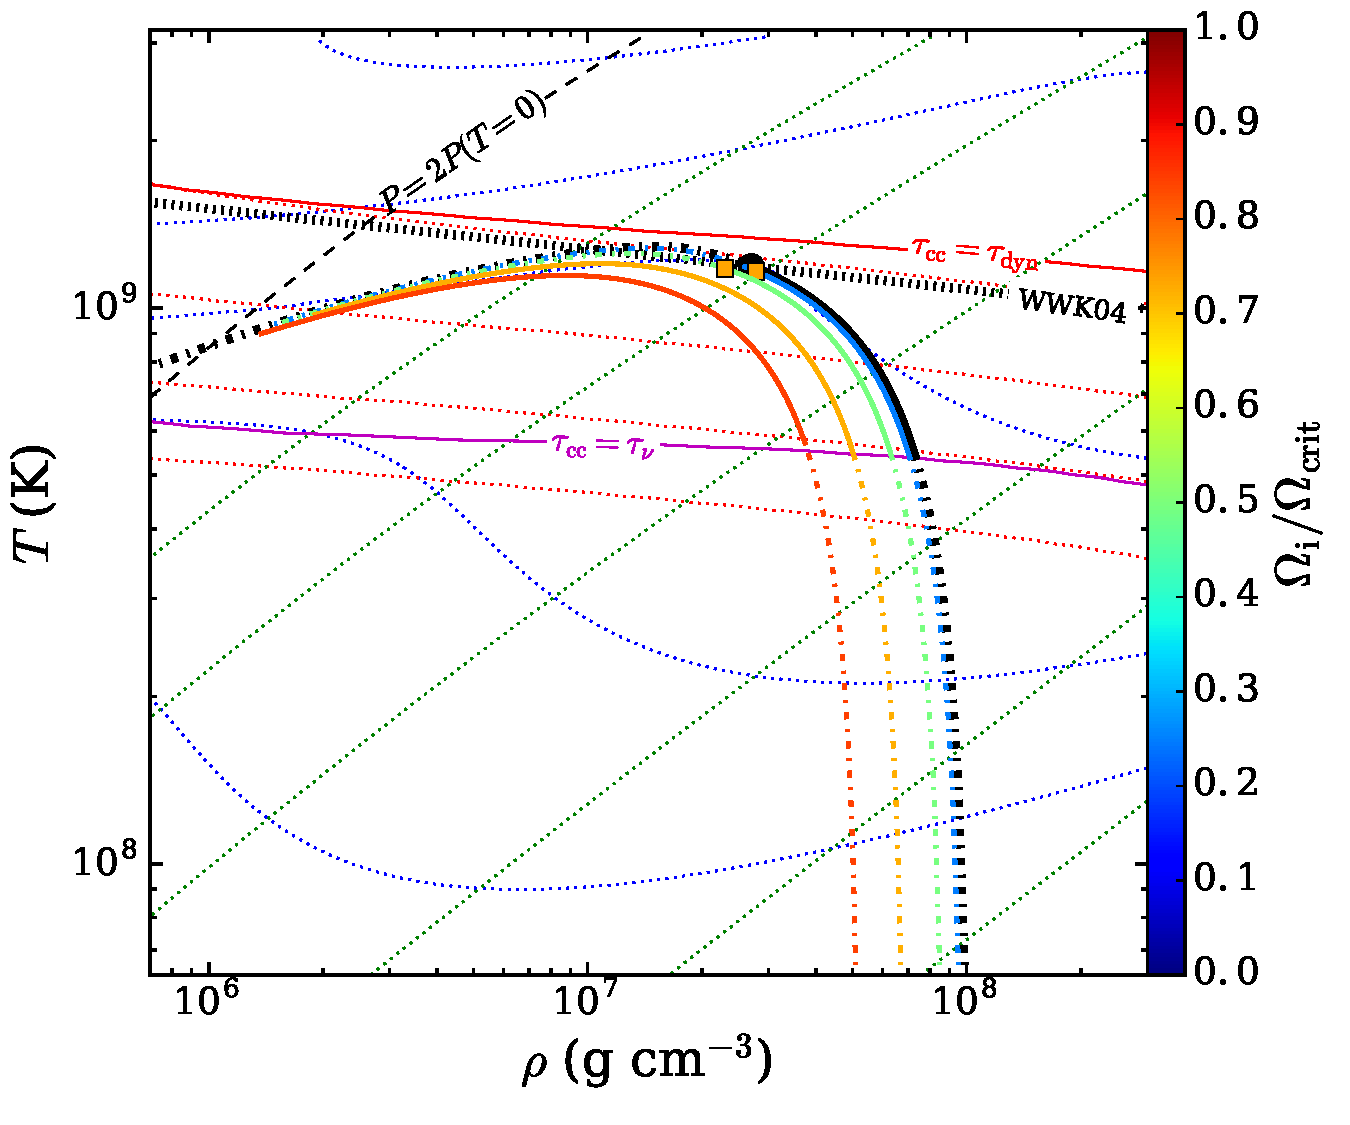
\includegraphics[angle=0,width=0.8\columnwidth]{chapter5_zhu+16/figures/rot_stev_1pt15_rhot.pdf}
\caption{simmering tracks for (unmagnetized) solid-body rotating $1.15\,\Msun$ WDs.  Track color represents $\Ominit/\Omcrit$, the ratio of the WD's angular speed at the start of simmering to its numerically determined break-up value, and the thicker black track is the non-rotating \dnabconv-inclusive $1.15\,\Msun$ one from Fig. \ref{fig:c5_runaway_rhot}.  \citeal{wooswk04} points are a black circle for the non-rotating track and orange squares for the rotating ones; the curves with $\Ominit/\Omcrit > 0.75$ never satisfy Eqn. \ref{eq:c5_endofsimmering}.  Dash-dotted track segments indicate solutions that cannot be reached during simmering.  All other lines and symbols are as in Fig. \ref{fig:c5_runaway_rhot}.}
\label{fig:c5_rot_stev_1pt15_rhot}
\end{figure}

%\eqbegin
%\deltanab_\mrm{GTSH} = \deltanab_\mrm{GT} + \deltanab_\mrm{SH}.
%\eqend

In Fig. \ref{fig:c5_rot_stev_1pt15_rhot}, we plot the simmering tracks of $1.15\,\Msun$ WDs with $\Ominit/\Omcrit$ varying from 25\% - 85\% of $\Omcrit = 0.61\,\mrm{s}^{-1}$ ($1.15\,\Msun$ is chosen for its proximity to the adiabatic \Mcrit\ value).  Below $10^{8}\,\mrm{K}$, the rotating WD tracks shift leftward (in density) from the non-rotating one (thick black line) -- from a factor of $0.03$ for $\Ominit/\Omcrit = 0.25$ to a factor of $1.9$ for $\Ominit/\Omcrit = 0.85$ -- due to centrifugal support supplementing degeneracy pressure.  This partial lifting of degeneracy competes with the convective suppression effects of rotation.  \citeal{stev79} notes the suppressive effect can be estimated by combining Eqns. \ref{eq:c5_superad_dev} and \ref{eq:c5_rot_nabrat_apx_low}:

\eqbegin
\dnabrot \approx 0.23\rossby^{-4/5}\dnabconvzero \sim \left(\frac{\Omega H_P}{\vconvzero}\right)^{4/5}\frac{\vconvzero^2}{g H_P} = \dnabconvzero^{3/5}\left(\frac{\Omega^2 H_P}{g}\right)^{2/5}.
\label{eq:c5_rot_limitapprox}
\eqend

\noindent All stars have $\Omega^2 H_P \lesssim g$, and so at best $\dnabrot \sim \dnabconvzero^{3/5}$.  For a $1.15\,\Msun$ WD rotating at less than a third of the critical rate, $\dnabconvzero \sim 10^{-2}$ near the end of simmering (Sec. \ref{ssec:c5_runaway_superad}) and $\dnabrot \lesssim 10^{-1.5}$, a $\lesssim10$\% deviation to \nablaad.  Our calculations give even more modest values: $\dnabrot/\nablaad \sim 0.03$ ($\dnabrot/\dnabconvzero \sim 1$) near the \citeal{wooswk04} point of both the $\Ominit/\Omcrit = 0.25$ and $\Ominit/\Omcrit = 0.50$ tracks.  These are lower than what Eqn. \ref{eq:c5_rot_limitapprox} predicts because for small values of $\Ominit$, $\rossby \sim 1$ near the end of simmering and Eqn. \ref{eq:c5_rot_nabrat_apx} approaches its non-rotating counterpart.  At the start of simmering, $\rossby \ll 1$ and $\dnabrot/\dnabconvzero \sim 200$ for the $\Ominit/\Omcrit = 0.50$ track, but $\dnabconvzero \sim 10^{-7}$ at this point, and so it makes little difference to the overall runaway.  Near critical rotation, Eqn. \ref{eq:c5_rot_limitapprox} predicts $\dnabrot \sim 10^{-1}$ which is more comparable to \nablaad, but our calculations show centrifugal support has a much larger effect on the runaway by lowering both \rhoc\ and \Tc\ of a model with a given \Sc.  This, in fact, reduces the effect of convective suppression by lowering \vconv.  This, rotation primarily serves to lift degeneracy and prevent a WD from reaching its \citeal{wooswk04} point.  At a modest $\Ominit/\Omcrit = 0.25$, the WD reaches its \citeal{wooswk04} point with $\rhoc = 2.8\times10^7\,\gcc$, only $\sim3$\% higher than its non-rotating counterpart.  As rotation increases, \rhoc\ at the \citeal{wooswk04} point decreases: it is $15$\% lower for the $\Ominit/\Omcrit = 0.50$ track, and tracks with higher rotation rates fail to reach the \citeal{wooswk04} point entirely.

The convective velocity, meanwhile, has a very shallow dependency on $\dnabrot/\dnabconvzero$.  At the end of simmering, $\vconvrcc = 1.1\times10^7\,\cmpsec$ for both the $\Ominit/\Omcrit = 0.25$ and $\Ominit/\Omcrit = 0.50$ tracks, comparable to the non-rotating value of $\vconvrcc = 1.3\times10^7\,\cmpsec$ (Sec. \ref{ssec:c5_runaway_superad}).  The $\sim20$\% difference in \vconvrcc\ is due to the sensitivity of \epscc\ and the \citeal{wooswk04} criterion to changes in temperature. 

%-- near the end of simmering small changes in temperature lead to large changes in \vconvrcc.

From the above analysis, it is unsurprising that a mass parameter space sweep for simmering WDs with $\Ominit/\Omcrit = 0.50$ yields $\Mcrit = 1.14\,\Msun$.  

%The corresponding $\MNi = 0.31\,\Msun$, though this is again much less well-constrained due to how much \rhoc\ changes near the simmering track turnover.  

Our results near critical rotation should be taken with a grain of salt, since deviations from spherical symmetry not reproducible by our model become significant. However, a merger remnant is unlikely to be critically rotating at the start of simmering.  As mentioned previously, studies of post-merger viscous evolution all find the remnant core spins down to well below critical rotation \citep{shen+12,schw+12,ji+13}.  While these works do not constrain the amount of vestigial rotation, we have shown above that modest rotation rates in general do little to influence the runaway.

\subsection{Simmering of Magnetized White Dwarfs}
\label{ssec:c5_runaway_mhd}

Like in the rotating case, the exact solution for the (dissipationless) magnetic case has no simple analytical form.  \citeal{stev79} finds in the limit of large Alfv\'{e}n ratio

\eqbegin
A = \frac{v_A^2}{\vconvzero^2} = \frac{B^2}{4\pi\rho\vconvzero^2}
\label{eq:c5_alfven_ratio}
\eqend

\noindent that \dnabmag\ and \vconv\ can be approximated as\footnote{We assume the magnetic field is aligned with the gravitational vector, and hence $\cos^2\phi = 1$ in Sec. 4 of \citeal{stev79}.  We have also corrected a coefficient error in \citeal{stev79}'s $\vconv/\vconvzero$ expression.}

%\noindent derived using an energy variation principle.  \Bv is the magnetic field in the radial direction and, as \cite{mullm01} notes, $\Bv(r)$ is a spherical mean-square averaging of the true field geometry.  In this work we only specify this spherically symmetric profile, and so drop the subscript with the understanding that the true 3D geometry may have significant $\hat{\theta}$ and $\hat{\phi}$ components.  For merger remnants, \cite{ji+13} and \cite{zhu+15}'s simulations both find the poloidal and toroidal field components in rough equipartition, suggesting \Bv\ is within a factor of $\sim2$ of field strength $B$.  $\gamma$ is the effective polytropic exponent, which we take to be \gammaad\ (the ratio of specific heats).  $1/\gamma_\mathrm{ad} = \alpha - \delta \nablaad$ and $\p\ln\rho/\p\ln P = \alpha - \delta\nabla$; combining these with Eqn. \ref{eq:gt66crit} gives  

%NOTES:
% - estimate of dynamo potential using R_m (Chabrier 2007 pg 2 paragraph 2)

\begin{eqnarray}
\frac{\dnabmag}{\dnabconvzero} &=& 0.24A \nonumber \\
\frac{\vconv}{\vconvzero} &=& 1.21A^{-1/2}
\label{eq:c5_mag_exactsoln}
\end{eqnarray}

\noindent Again, in lieu of solving for $\dnabmag/\dnabconvzero$ exactly during integration, we use the approximations 

\begin{eqnarray}
\frac{\dnabmag}{\dnabconvzero} &\approx& \left(1 + \left(0.24A\right)^{6/5}\right)^{5/6}, \nonumber \\
\frac{\vconv}{\vconvzero} &\approx& \left(1 + \left(1.21A^{-1/2}\right)^{-13/4}\right)^{-4/13}.
\label{eq:c5_mag_apx}
\end{eqnarray}

\noindent Exponents $6/5$ and $-13/4$ were obtained by empirically minimizing these functional forms to the numerically calculated exact solutions over a range $10^{-4} < A < 10^4$.  $\dnabmag/\dnabconvzero$ in Eqn. \ref{eq:c5_mag_apx} is accurate to within $2$\% of its exact solution, and $\vconv/\vconvzero$ to within $3$\%.  We assume the magnetic field is frozen to its corresponding mass shell $m$ throughout the runaway, changing in strength to satisfy conservation of flux $d\Phi \propto B r^2$ (i.e. $B(m) \propto 1/r(m)^2$), meaning that, analagous to the rotation case above, the magnetic field only needs to be specified for one model in the runaway.  We again take the \Sc\ of this model to be that for the first model above the ignition line in the equivalent adiabatic simmering track.  We set the initial field profile $B_0(m)$ to be one where

\eqbegin
\dmag = \frac{B_0^2}{8\pi P}
\label{eq:c5_cdev}
\eqend

% papercalc_arepo.py plots the spherical field profile of the 0.625 - 0.65 Msun remnant at 200, 600 and 1000 s after coalescence - we see that the B vs. m profile vaguely in broad strokes looks similar to a \dmag profile for a hydrostatic WD, but the \dmag vs. m profile increases with radius, peaking at ~0.7M_tot and then decreasing sharply.  We shouldn't take these comparisons too seriously, since we cannot compare a non-rotating equilibrated WD with a rotating one recently birthed from a merger.

\noindent is held constant, suggested by \cite{macdm09}, who use it to study magnetic convective suppression in brown dwarfs, as a reasonable profile for a star whose density does not vary wildly over most of its interior.  The spherically averaged magnetic field profile of the merger remnant in \cite{zhu+15} also resembles Eqn. \ref{eq:c5_cdev} near the center of its core, though caution must be used comparing a recently formed merger remnant with a hydrostatic simmering WD.  The central initial field strength \Binit\ is restricted to below $10^{12}\,\mrm{G}$ to keep $\dmag \ll 1$ ($\dmag = 0.01$ when $\Binit = 2.0\times10^{12}\,\mrm{G}$ for a $1.15\,\Msun$ WD at the ignition line).  This allows us to leave out magnetic terms in Eqn. \ref{eq:c5_hydroeq}.

%As we know of no reasonable scenario to form a WD where $\Pmag/\Pgas \sim 0.1 - 1$, even in a process as violent as a merger \citep{vkercj10,wicktf14,ji+13, zhu+15}, this is unlikely to be a prohibitive restriction.

\begin{figure}
\centering
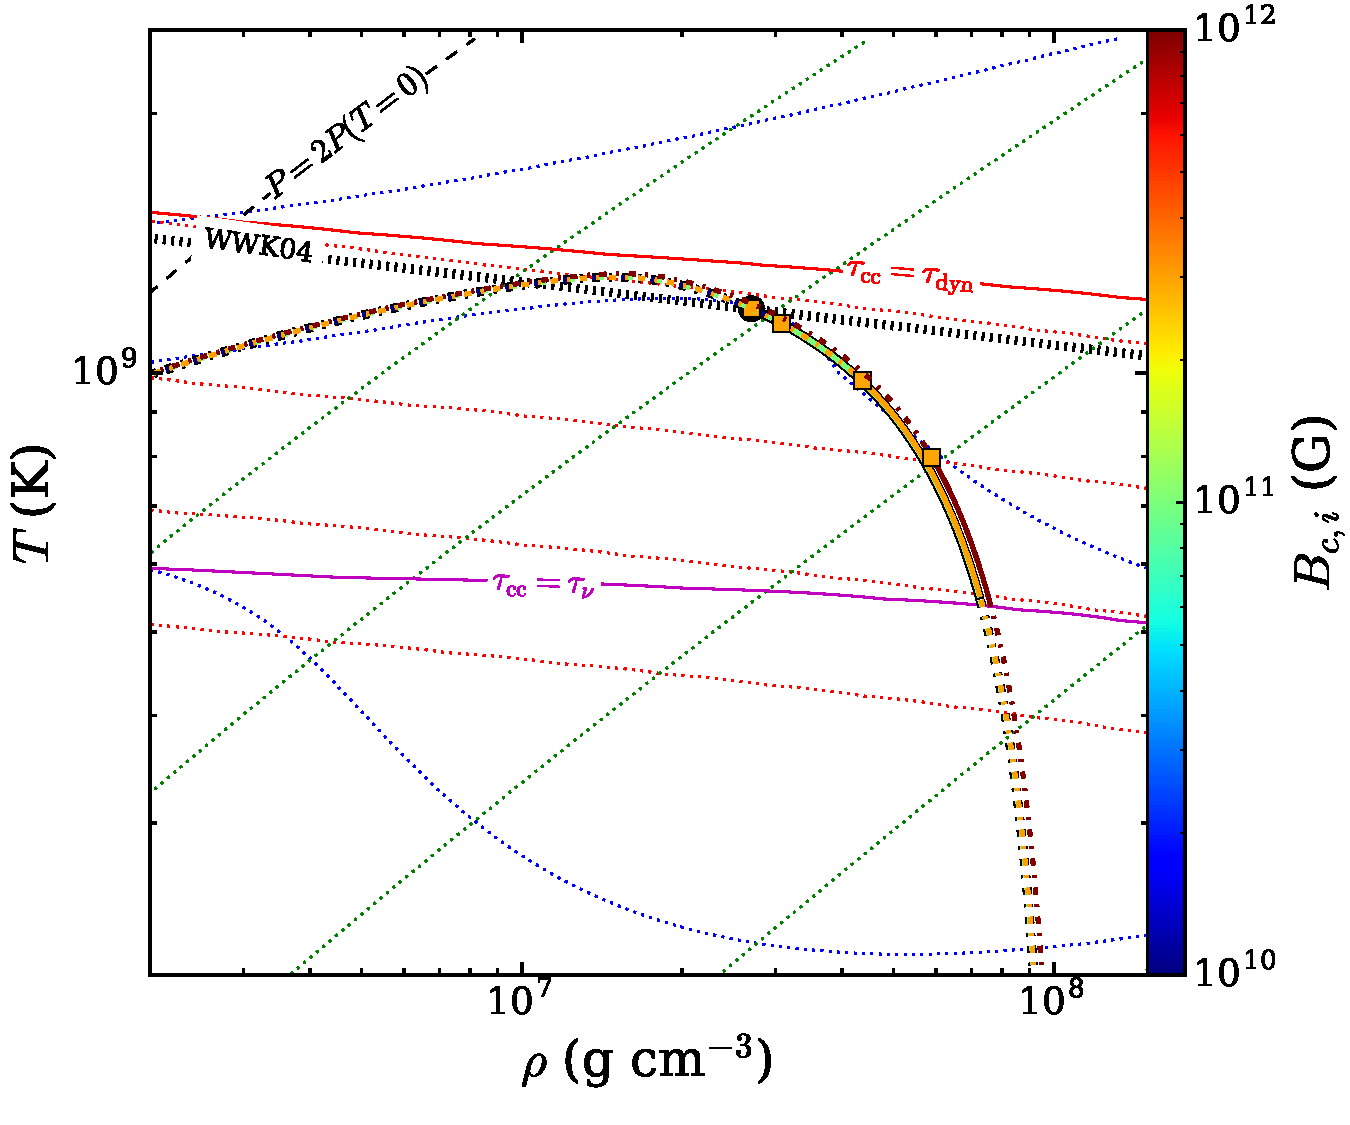
\includegraphics[angle=0,width=0.8\columnwidth]{chapter5_zhu+16/figures/mag_1pt15_rhot.pdf}
\caption{simmering tracks for (non-rotating) magnetized $1.15\,\Msun$ WDs.  Track color represents the central magnetic field strength at the start of simmering, \Binit, and the thicker black dotted track is the non-magnetized \dnabconv-inclusive $1.15\,\Msun$ one from Fig. \ref{fig:c5_runaway_rhot}.  All other lines and symbols are as in Fig. \ref{fig:c5_rot_stev_1pt15_rhot}, except that the orange circles represent \citeal{wooswk04} points for the magnetized (rather than rotating) tracks.}
\label{fig:c5_mag_1pt15_rhot}
\end{figure}

Fig. \ref{fig:c5_mag_1pt15_rhot} depicts simmering tracks for a $1.15\,\Msun$ with $\Binit = 1\times10^{10}-1\times10^{12}\,\mrm{G}$.  Across the entire range of field strengths, the shift in the simmering track shape due to \dnabmag\ is small.  The \rhoc\ values of the magnetized tracks deviate by $\lesssim5$\% from the non-magnetized one, even for the strongest field strengths being considered.  This is because, for $A \gg 1$, Eqn. \ref{eq:c5_mag_exactsoln} can be rewritten as

\eqbegin
\dnabmag \approx \frac{1}{\delta}\frac{B^2}{16\pi \rho g H_P} = \frac{1}{\delta}\frac{B^2}{16\pi P},
\label{eq:c5_mag_apx_high}
\eqend

\noindent or $\dmag/2\delta$.  Note that Eqn. \ref{eq:c5_mag_apx_high} is identical to Eqn. \ref{eq:c5_dnabmag_est}, obtained by balancing the buoyancy and Lorentz forces, and a similar expression is derived in \cite{macdm09} based on one from \cite{gougt66}.  Since we consider fields with $\dmag < 3\times10^{-3}$, \dnabmag\ is large only when $1/\delta$ is.  This is the case close to the $\taucc = \taunu$ line, leading to $\dnabmag/\nablaad \sim 0.2$ for the $\Binit = 10^{12}\,\mrm{G}$ track, but for colder and highly degenerate WDs their temperature profile has little influence on their density profile.  When $T\gtrsim10^9\,\mrm{K}$, $1/\delta$ is much smaller and \dnabmag\ approaches \dnabconv\ in value.

\vconv, however, is proportional to $A^{-1/2}$ when $A \gg 1$, and can be many orders of magnitude smaller than \vconvzero\ during the earlier phases of simmering.  For the $\Binit = 1\times10^{12}\,\mrm{G}$ track, \vconv\ is reduced so much that Eqn. \ref{eq:c5_endofsimmering} is satisfied at $\rhoc = 5.9\times10^7\,\gcc$, $\Tc = 8.0\times10^8\,\mrm{K}$, well-below the adiabatic \citeal{wooswk04} line.  At the \citeal{wooswk04} point for the $\Binit = 1\times10^{12}\,\mrm{G}$ run, $A \sim 3\times10^3$, and hence $\vconvrcc = 1.3\times10^{4}\,\cmpsec$, a factor of $\sim30$ smaller than \vconvzero\ and $\sim10^3$ smaller than \vconvrcc\ at the end of simmering for the unmagnetized track.  This reduction appears only for $\Binit \gtrsim 3\times10^{11}\,\mrm{G}$; for the $\Binit = 1\times10^{11}\,\mrm{G}$ one, simmering ends when $A \sim 10^{-1}$, and \rhoc\ and \Tc\ deviate from from their non-rotating values by $14$\% and $4$\%, respectively.

%at $\rhoc = 3.1\times10^7\,\gcc$, $\Tc = 1.1\times10^9\,\mrm{K}$

We perform a parameter space search of WDs with either low or high-strength magnetic fields.  Strength is defined as the magnetic to total energy ratio \EBEtot; ``Low'' means $\EBEtot = 2.9\times10^{-5}$ and ``high'' means $\EBEtot = 2.8\times10^{-3}$, equivalent to $\Binit = 1\times10^{11}\,\mrm{G}$ and $\Binit = 1\times10^{12}\,\mrm{G}$, respectively, for a $1.15\,\Msun$ WD.  Similar to the non-rotating case, the low field search yields $\Mcrit = 1.13\,\Msun$.  The high field search yields $\Mcrit = 1.02\,\Msun$, a reduction of more than $0.1\,\Msun$ from the non-magnetized case.  The latter estimates are the most uncertain out of all those in this work, which is discussed at length in the main paper.  

%and $\MNi = 0.21\,\Msun$

%\MNi\ grows from $\MNi = 0.26$ for $1.05\,\Msun$ to $\MNi = 0.75\,\Msun$ for $1.15\,\Msun$.  The latter value is around twice \MNi\ of the unmagnetized $1.15\,\Msun$ simmering track because the \citeal{wooswk04} point occurs so much earlier in the magnetized case, before the WD has the chance to expand significantly from its zero-temperature density structure.

%and \MNi\ rapidly grows to $0.51\,\Msun$ for a $1.15\,\Msun$ WD

However, we have already mentioned in Sec. \ref{ssec:c5_magaccuracy} that these results, particularly those at the high-field limit, must be treated with caution.  \citeal{stev79}'s magnetic formulation has not yet been numerically tested and may not accurately reflect non-linear magnetoconvection, except perhaps in the case of weak fields.  Moreover, dynamo processes are likely to be efficient in simmering WDs and will likely lead to $\sim10^{12}\,\mrm{G}$ fields near the end of simmering, dominating over any fossil fields from prior evolution.

%Our \Mcrit\ and \MNi\ values are instead estimates of the maximum possible effect, equivalent to assuming the simmering track becomes vertical once reaching the \citeal{wooswk04} point.  While our results then show that extremely strong magnetic fields can potentially reduce \Mcrit\ by more than $0.1\,\Msun$, $10^{12}$ G is more than an order of magnitude higher than the peak field strength produced during or after a merger \citep{ji+13,zhu+15}.  A $10^{11}\,\mrm{G}$ field is likely to be more realistic, and results in a much less extreme deviation from the non-rotating case.

%We have thus shown that the simmering track for a WD with reasonable rotation rates or magnetic field strengths deviates by $\lesssim10$\% for all values, except \MNi, from its non-rotating and unmagnetized counterpart.  The non-rotating, unmagnetized runaway itself is well-approximated by an adiabatic simmering track.

%A field of $1\times10^{12}\,\mrm{G}$ is also $\sim30$ times greater than the average strength within the core of the remnant reported in the simulations of \cite{ji+13} and \cite{zhu+15}.\footnote{The total magnetic energies reported from both simulations are also a factor of $\gtrsim20$ smaller those of the $1\times10^{12}\,\mrm{G}$ tracks, but this is much harder to compare due to the density and magnetic field structures in the  simulations extending far from the remnant core.}  The value of $B^2/(B^2 + 4\pi\gamma P)$ must remain low for more realistic magnetic field strengths, making any changes to the runaway process likely to be minor.  Indeed, \Binit\ must remain $\lesssim3\times10^{11}\,\mrm{G}$ for a uniform field and $\lesssim2\times10^{12}\,\mrm{G}$ for a constant \dmag\ field to keep the ratio of magnetic to degeneracy pressure $P_\mrm{mag}/P_\mrm{deg} \lesssim 10^{-2}$ throughout the WD.

\subsection{Sensitivity to Mixing Length Theory Coefficients}
\label{ssec:c5_sensitive_apdx}

We noted above that that \citeal{stev79}'s formulation reproduced the equations of MLT in the non-rotating, unmagnetized limit, except for differing prefactor coefficients, and that to reproduce the properties of the Sun it had to further be calibrated by setting $l_m \sim 3$.  Both $l_m$ and the coefficients vary among different formulations of convection.  To get a sense of the robustness of our estimate for \Mcrit\ and \MNi\ to these variations, we generate a simmering track for a $1.15\,\Msun$ WD where we replace the ``default'' Eqns. \ref{eq:c5_vconv_mlt} and \ref{eq:c5_superad_dev} with Eqns. \ref{eq:c5_vconv_stev} and \ref{eq:c5_superad_dev_stev}, respectively, and set $l_m = 3$.  This is practically equivalent to rescaling \vconv\ by a factor of $0.85$, and $\nabla$ by a factor of $3.26$.

%\eqbegin
%\Fconv = \frac{4\pi}{25}\left(\frac{5}{2}\right)^{5/2}\frac{\rho c_PT}{\gacc\delta l_m} \vconv^3,
%\label{eq:vconv_stevcal}
%\eqend

%\eqbegin
%\dnabconv = \frac{25\pi^2}{6}\frac{\vconv^2}{\gacc\delta}\frac{H_P}{l_m^2}.
%\label{eq:superad_dev_stevcal}
%\eqend

%\noindent in lieu of Eqns. \ref{eq:vconv_mlt} and \ref{eq:superad_dev}.

\begin{figure}
\centering
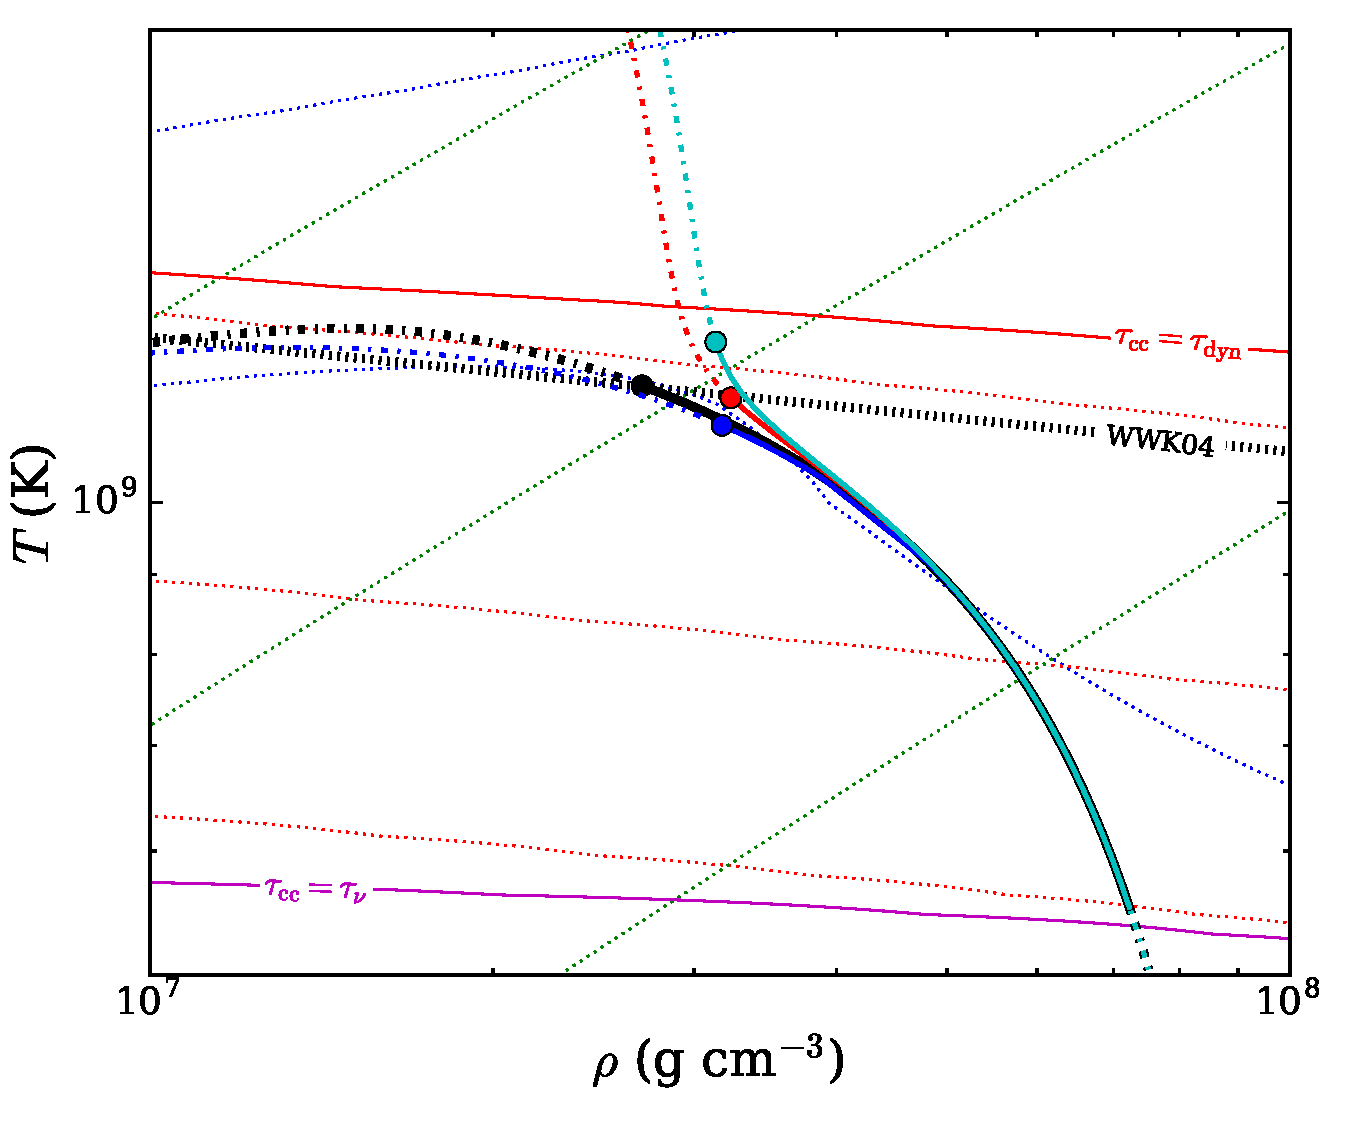
\includegraphics[angle=0,width=0.8\columnwidth]{chapter5_zhu+16/figures/diag_1pt15_rhot.pdf}
\caption{Comparison of a simmering track for a non-rotating, unmagnetized $1.15\,\Msun$ WDs calculated using Eqns. \ref{eq:c5_vconv_stev} and \ref{eq:c5_superad_dev_stev} (red line) with the ``default'' $1.15\,\Msun$ one that uses Eqns. \ref{eq:c5_vconv_mlt} and \ref{eq:c5_superad_dev} from Fig. \ref{fig:runaway_rhot} (black).  Also plotted are tracks which use Eqn. \ref{eq:c5_superad_dev} but multiply a prefactor of $2$ (blue) or $1/2$ (cyan) to Eqn. \ref{eq:c5_vconv_mlt}.  Circles along each track indicate their respective \citeal{wooswk04} points.  All other lines and symbols are as in Fig. \ref{fig:c5_rot_stev_1pt15_rhot}.}
\label{fig:c5_mltcoeff_rhot}
\end{figure}

In Fig. \ref{fig:mltcoeff_rhot}, we compare the \citeal{stev79} coefficient (SC; solid red line) track with the one using default coefficients (solid black).  There is little difference between the two lines until close to the end of simmering, where increased superadiabaticity leads to a steepening of the SC track; it ends simmering with $20$\% higher \rhoc.  Adding $50$\% critical rotation or a $10^{11}$ G magnetic field yields additional deviations of $\sim10$\% in \rhoc\ near the end of simmering.  A mass parameter-space search of \Mcrit\ for the SC tracks yields $\Mcrit = 1.12\,\Msun$, a deviation on par with those seen in previous sections.

%($\MNi = 0.2\,\Msun$)

The \citeal{stev79} coefficients only modify \vconv\ by $15$\%, so the deviations above are due to the change in \deltanab.  Since Eqn. \ref{eq:c5_superad_dev} also depends on \vconv, modifying it can result in comparable changes.  In Fig. \ref{fig:mltcoeff_rhot} we show tracks calculated using Eqn. \ref{eq:c5_superad_dev} as is, but multiply a factor of $2$ (``$2v$''; blue dashed) or $1/2$ (``$v/2$''; cyan dashed) to Eqn. \ref{eq:c5_vconv_mlt}.  The larger \deltanab\ in the $2v$ track leads it to steepen near the end of simmering like the SC one, while the $v/2$ track more resembles the adiabatic one in Fig. \ref{fig:runaway_rhot}.  Altering \vconv\ also changes where Eqn. \ref{eq:c5_endofsimmering} is satisfied.  The $v/2$ track reaches its \citeal{wooswk04} point when $\vconvrcc = 4.4\times10^6\,\cmpsec$ and with $18$\% higher \rhoc\ ($6$\% lower \Tc), than the default track; the $2v$ track ends simmering when $\vconvrcc = 4.3\times10^7\,\cmpsec$, but also with $16$\% higher \rhoc\ ($7$\% higher \Tc) due to it being steeper.  A search of \Mcrit\ for $v/2$ and $2v$ tracks both give $\Mcrit = 1.12\,\Msun$.

%(($\MNi = 0.15\,\Msun$) for $v/2$, $\MNi = 0.2\,\Msun$ for $2v$).

%The combined effects a modified prescription and near-critical rotation or a much stronger magnetic field are more substantive (since the effects of the latter two are also multiplicative): while, for example, while the default coefficient $10^{12}$ G simmering track in Fig. \ref{fig:mag_1pt15_rho} closely follows its non-magnetized counterpart, the SC $10^{12}$ G track deviates by a factor of 10\% in \rhoc\ throughout its simmering track.  As discussed in Sec. \ref{ssec:runaway_mhd}, however, we believe our $10^{12}$ G models to be less reliable, and for $10^{12}$ G fields to unlikely even for a merger remnant.

We thus find that changing MLT coefficients leads to changes in the simmering tracks and to \Mcrit\ on par with including the convective superadiabaticity \dnabconv\ in Sec. \ref{ssec:runaway_superad}.  Likewise, these deviations are also ultimately too small to significantly change our results.

%making more accurate modelling of convection at the end of simmering, as important to determining the fate of simmering WDs.

%but ones that are as large, or larger than, the changes seen when switching from the adiabatic approximation to more complex formulations, including adding rotation and magnetic fields, in previous sections.  Accurately modelling convection close to the end of simmering, then, is likely to be as or more important to determining the fate of simmering WDs as including rotation or magnetic fields from prior evolution.

